\documentclass[12pt,a4paper,titlepage]{article}

\usepackage{preamble}

\title{Fetal ECG extraction}
\author{Yassine Jamoud, Samy Haffoudhi}
\date{\today}

\begin{document}

\maketitle

\section*{Introduction}

Le but de ce TP est d'extraire un ECG fœtal à partir de mesures issues de capteurs abdominaux.
Nous allons commencer par l'analyse et la détection de pics R d'un ECG sain. Puis nous 
passerons à l'extraction d'un ECG fœtal en implémentant deux méthodes complémentaires : 
le filtrage spatial par PCA (periodic component analysis ) et le filtre de Kalman étendu.

\section{Healthy ECG signal analysis}

\subsection{Basic analysis}

Commençons par représenter le signal ECG considéré:

\begin{figure}[H]
    \caption{Signal ECG}
    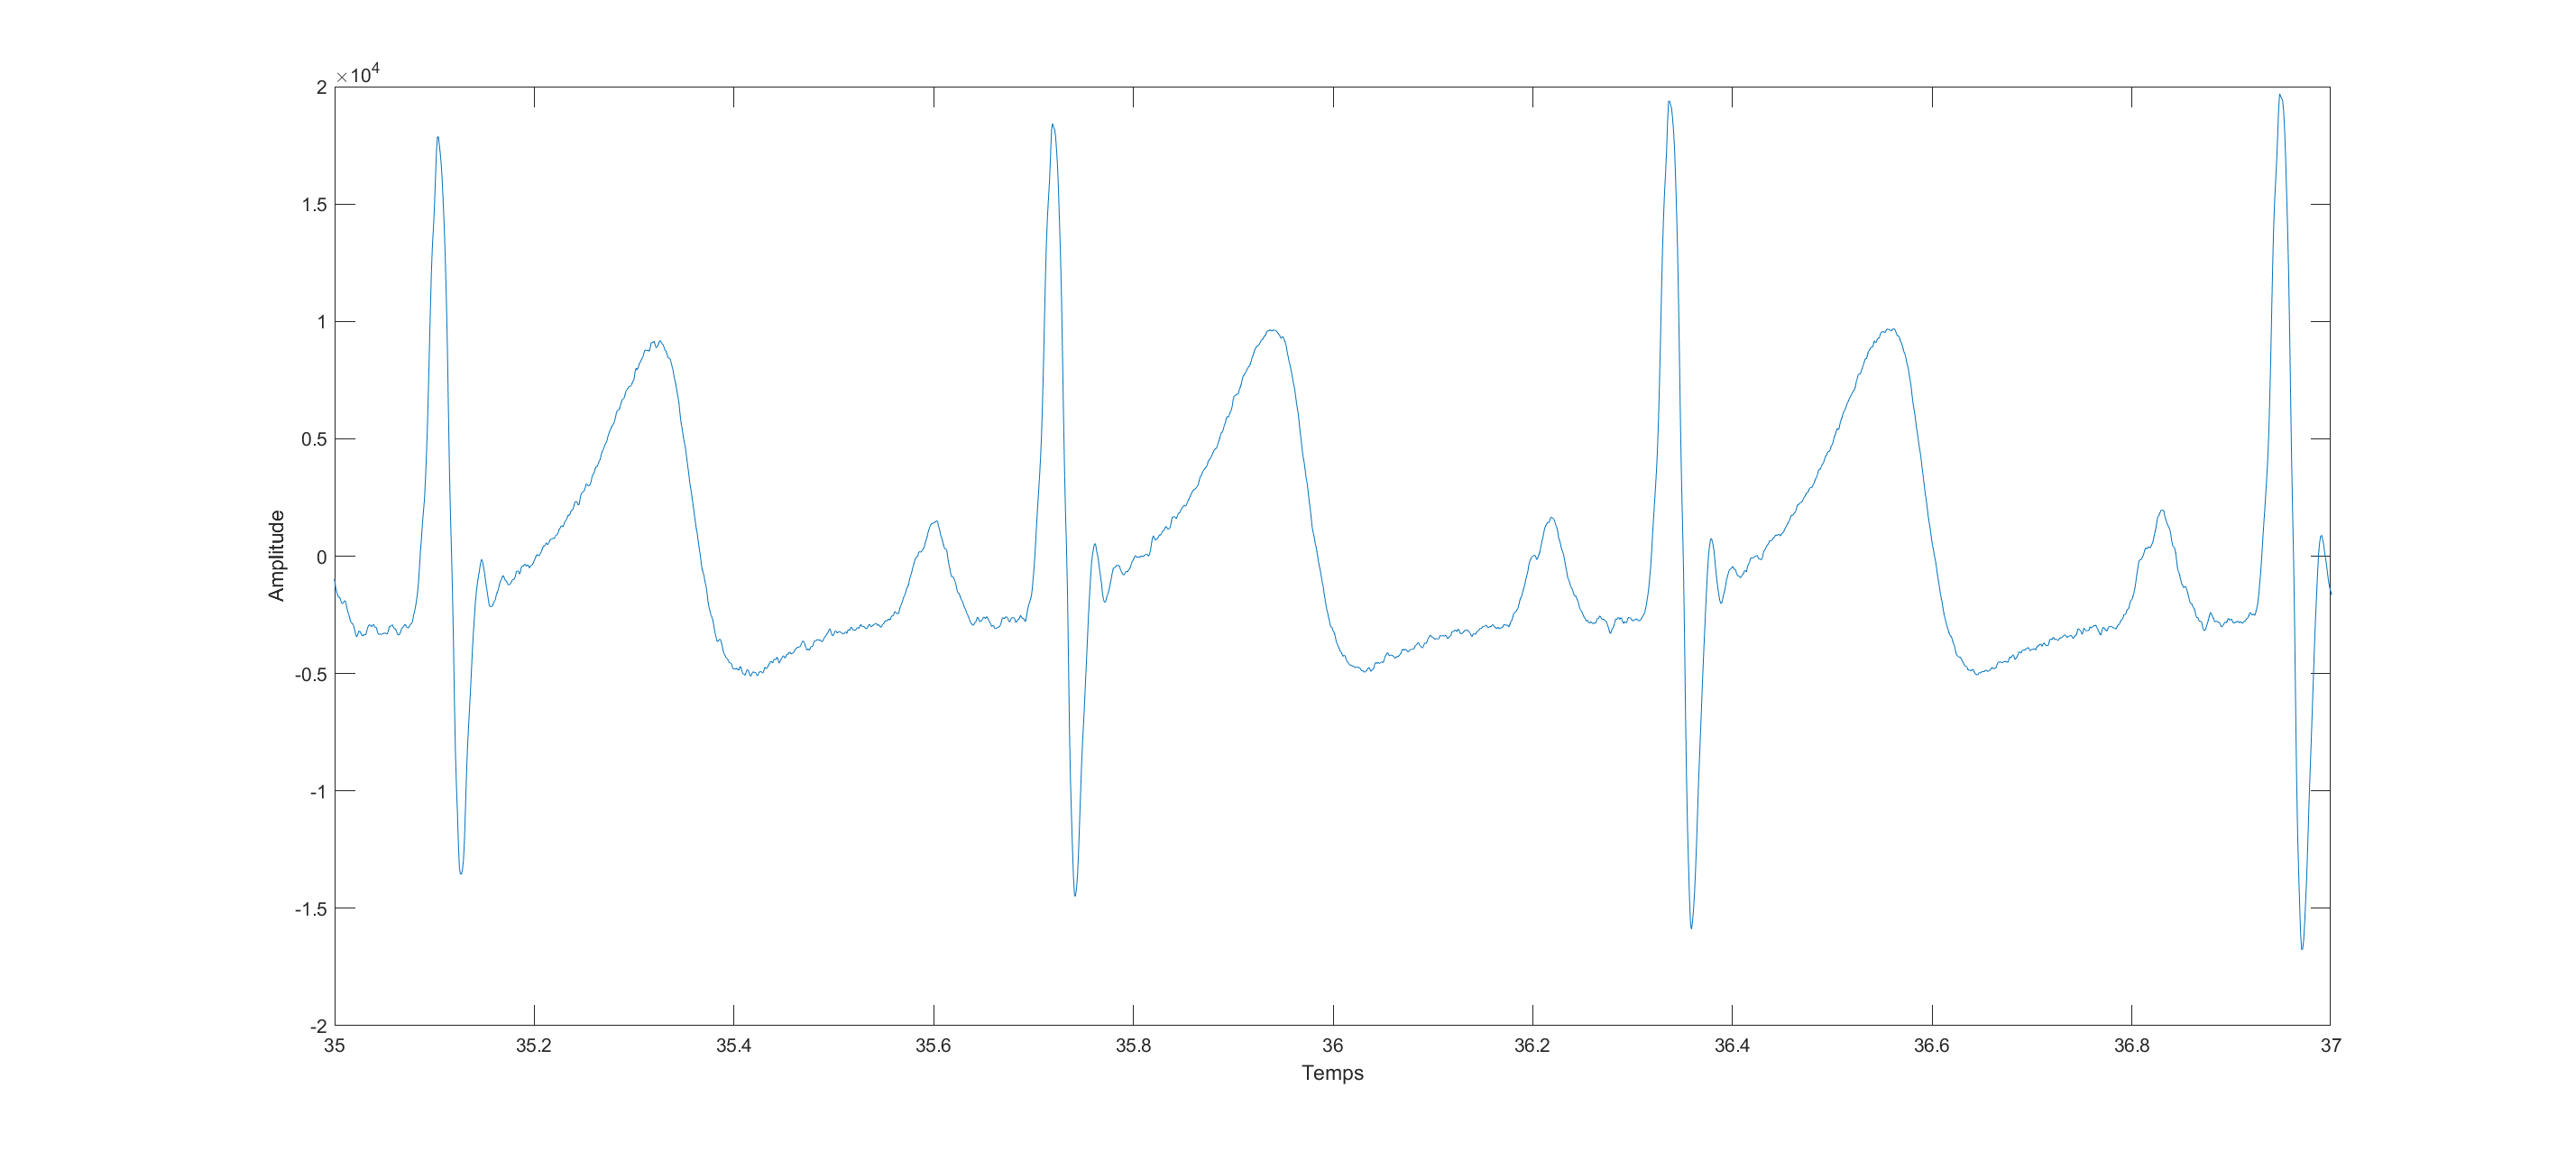
\includegraphics[width=\textwidth]{fig1}
    \centering
\end{figure}

On reconnait bien l'allure générale d'un ECG sain. On peut en particulier, distinguer les 
différentes ondes et observer la quasi-périodicité du spectre.

Représentons le spectre associé :

\begin{figure}[H]
    \caption{Spectre de l'ECG}
    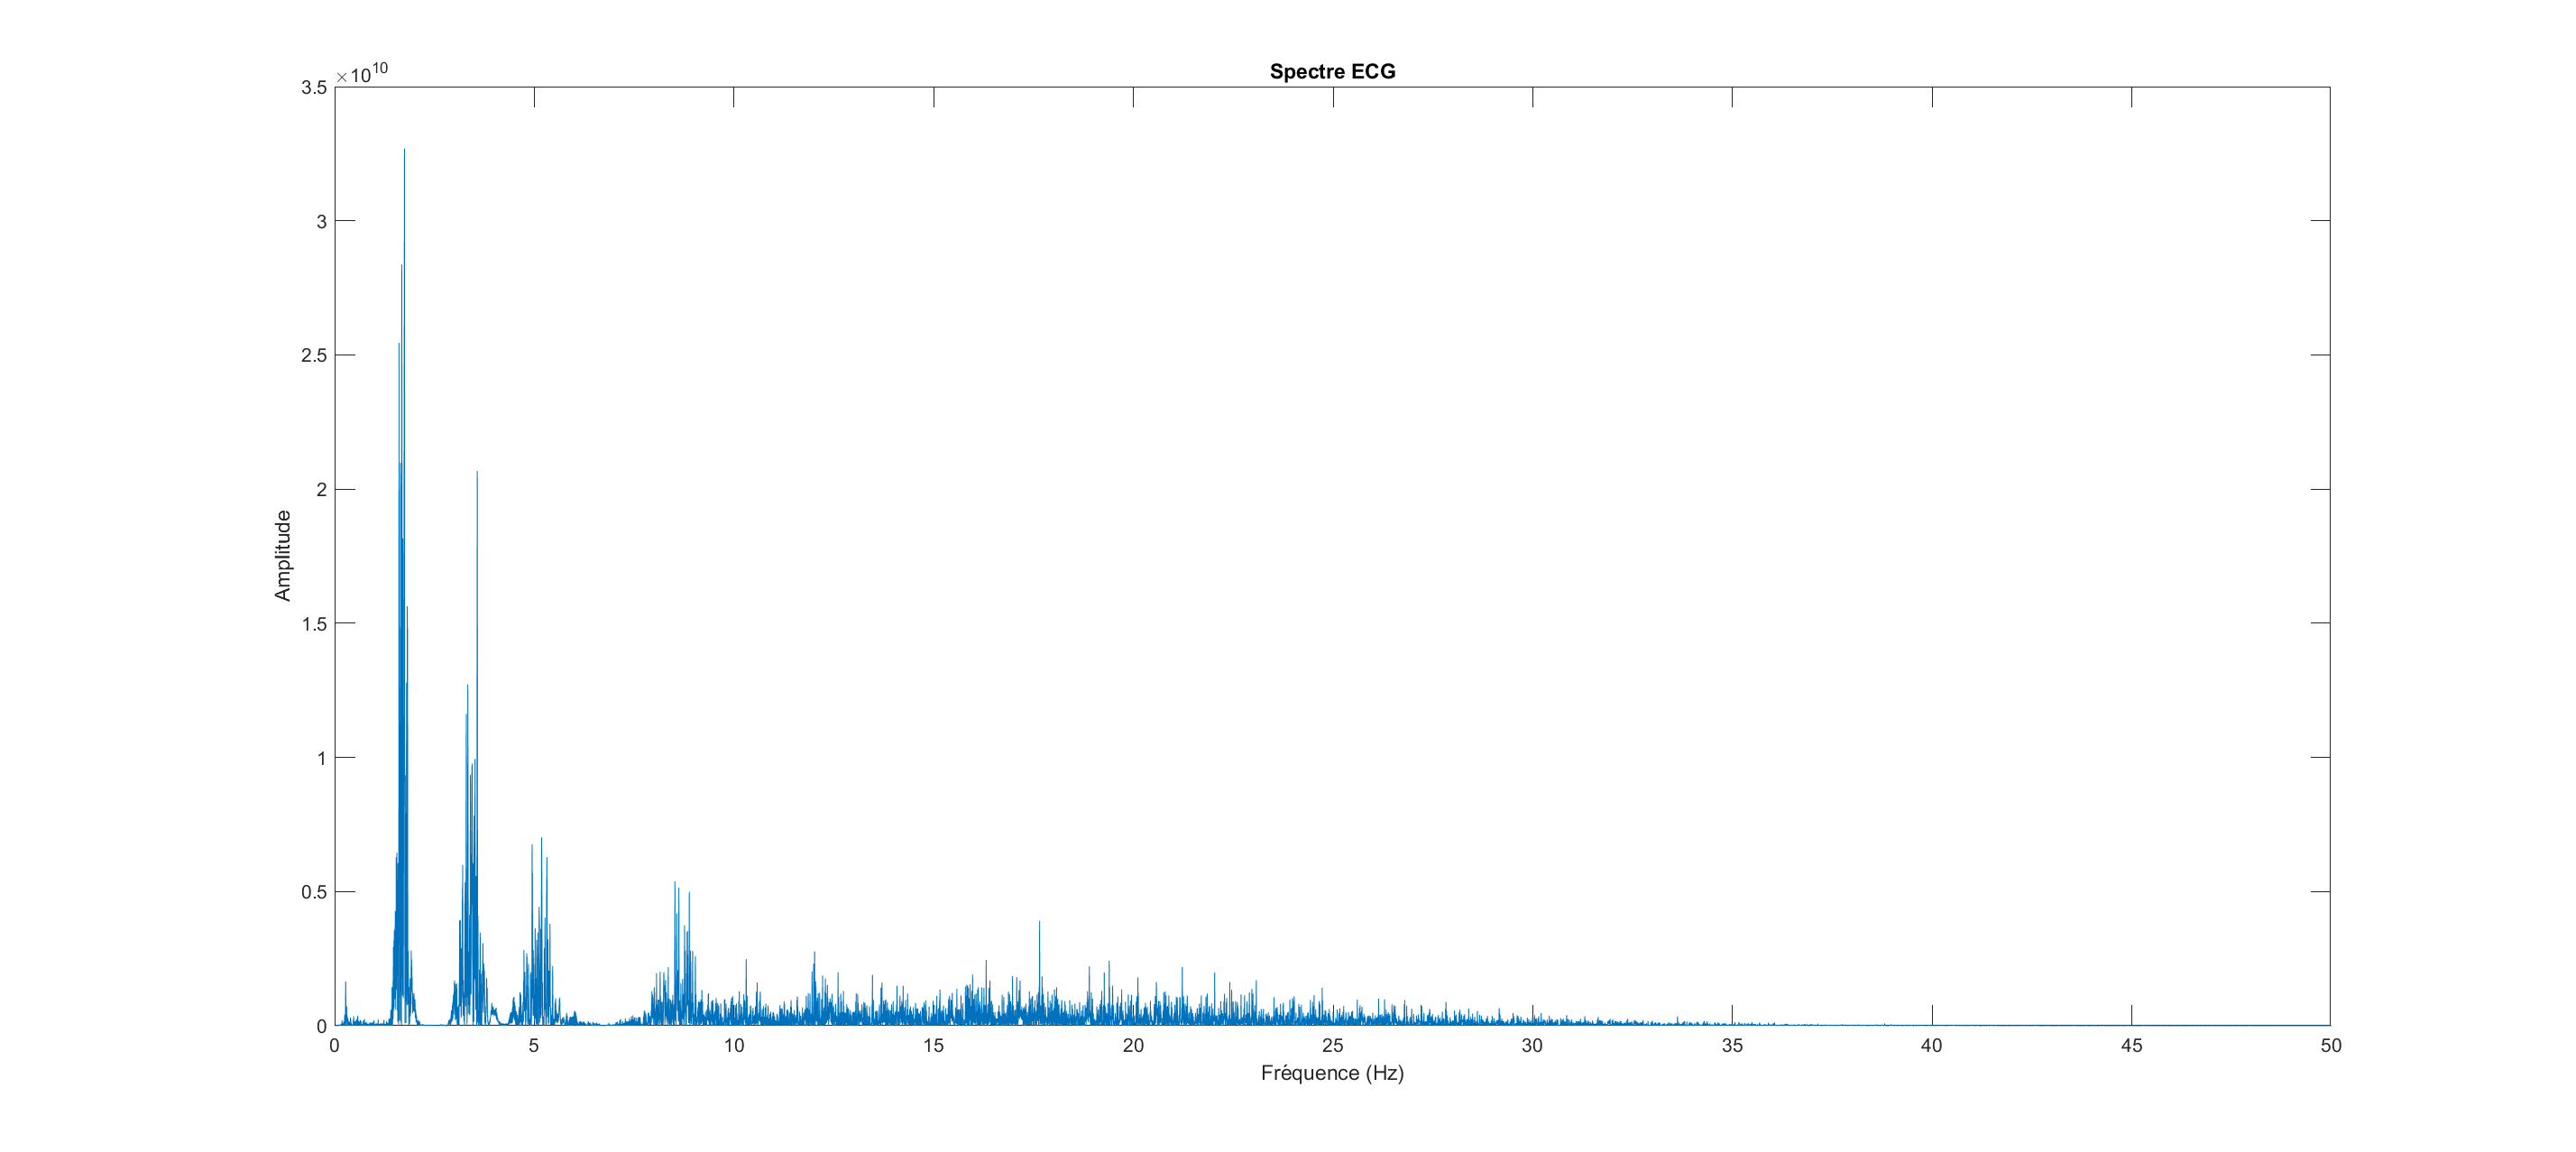
\includegraphics[width=\textwidth]{fig2}
    \centering
\end{figure}

On remarque que les composantes fréquentielles du signal correspondent à de basses
fréquences, on se restreint à un tracé du spectre entre 0 et 50 Hz. Par ailleurs, les
amplitudes sont globalement décroissantes avec la fréquence et le spectre s'apparente 
à un peigne de Dirac, ce qui s'explique par la quasi-périodicité du signal.

Le spectre ne permettant pas d'obtenir des informations temporelles, on s'intéresse 
maintenant au spectrogramme du signal.

Représentons le spectrogramme pour trois choix différents de taille de fenêtre :

\begin{figure}[H]
    \caption{Spectrogramme de l'ECG}
    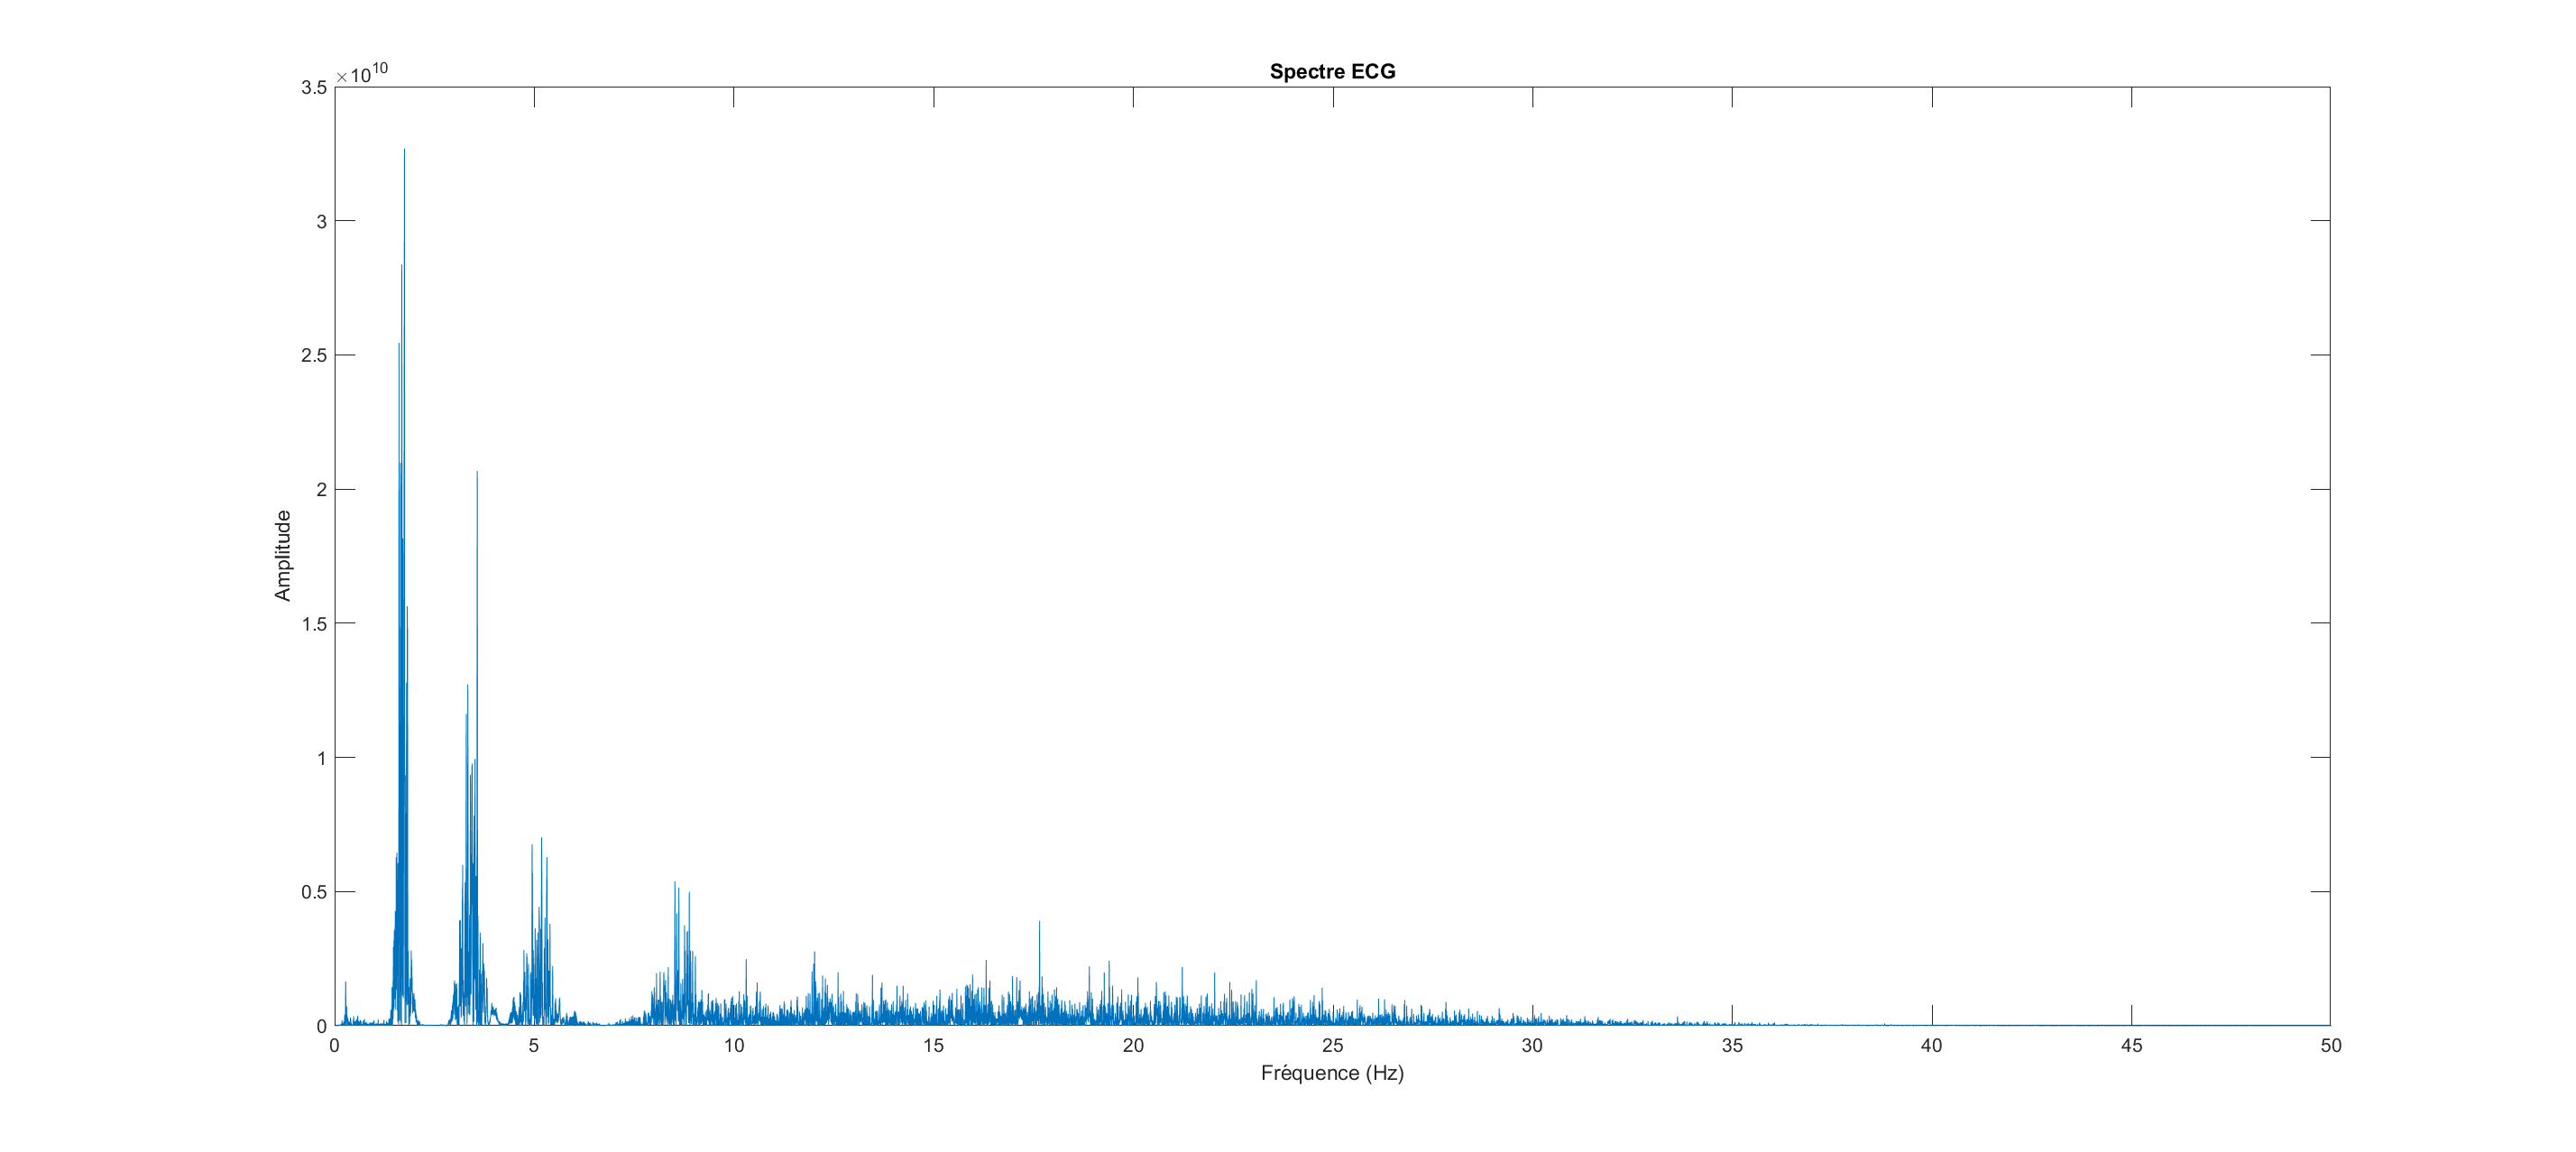
\includegraphics[width=\textwidth]{fig2}
    \centering
\end{figure}

On peut observer l'influence de la taille de la fenêtre sur l'allure du spectrogramme obtenu.
En effet, pour une fenêtre plus courte, d'une durée de 150ms, on observe un étalement en fréquences tandis que
pour une durée plus importante, 2s, on a cette fois un étalement moins important en fréquences.
Cette dualité temps-fréquence nécessite alors un choix de paramètre adapté à l'information
recherchée sur le spectrogramme.

\subsection{R peak detection}

\subsubsection{Design and analysis of filters}

Le processus de détection des pics R repose sur l'utilisation de plusieurs filtres.

\begin{itemize}
    \item{Un filtre passe-bas : $H(z) = \frac{(1-z^{-n})^2}{(1-z^{-1})^2}$ avec
        $n = \frac{F_s}{F_c} = \frac{1000}{40} = 25$}
    \item{Un filtre passe-haut : $H(z) = nz^{-\frac{n-1}{2}} - \frac{1-z^{-1}}{1-z^{-1}}$
        avec $n = \frac{F_s}{F_c} =\frac{1000}{8} = 125$.}
    \item{Un filtre dérivateur}
    \item{Un filtre MA : $H(z) = \frac{1}{n} \frac{1-z^{-n}}{1-z^{-1}}$ avec 
            $n = 149$. En effet, pour $F_s$ = 200 Hz, les auteurs de l'article ont $n = 30$,
        on choisit 149 pour obtenir n impair.}
\end{itemize}

Représentons les réponses des différents filtres :

\begin{figure}
\begin{subfigure}{.5\textwidth}
  \centering
  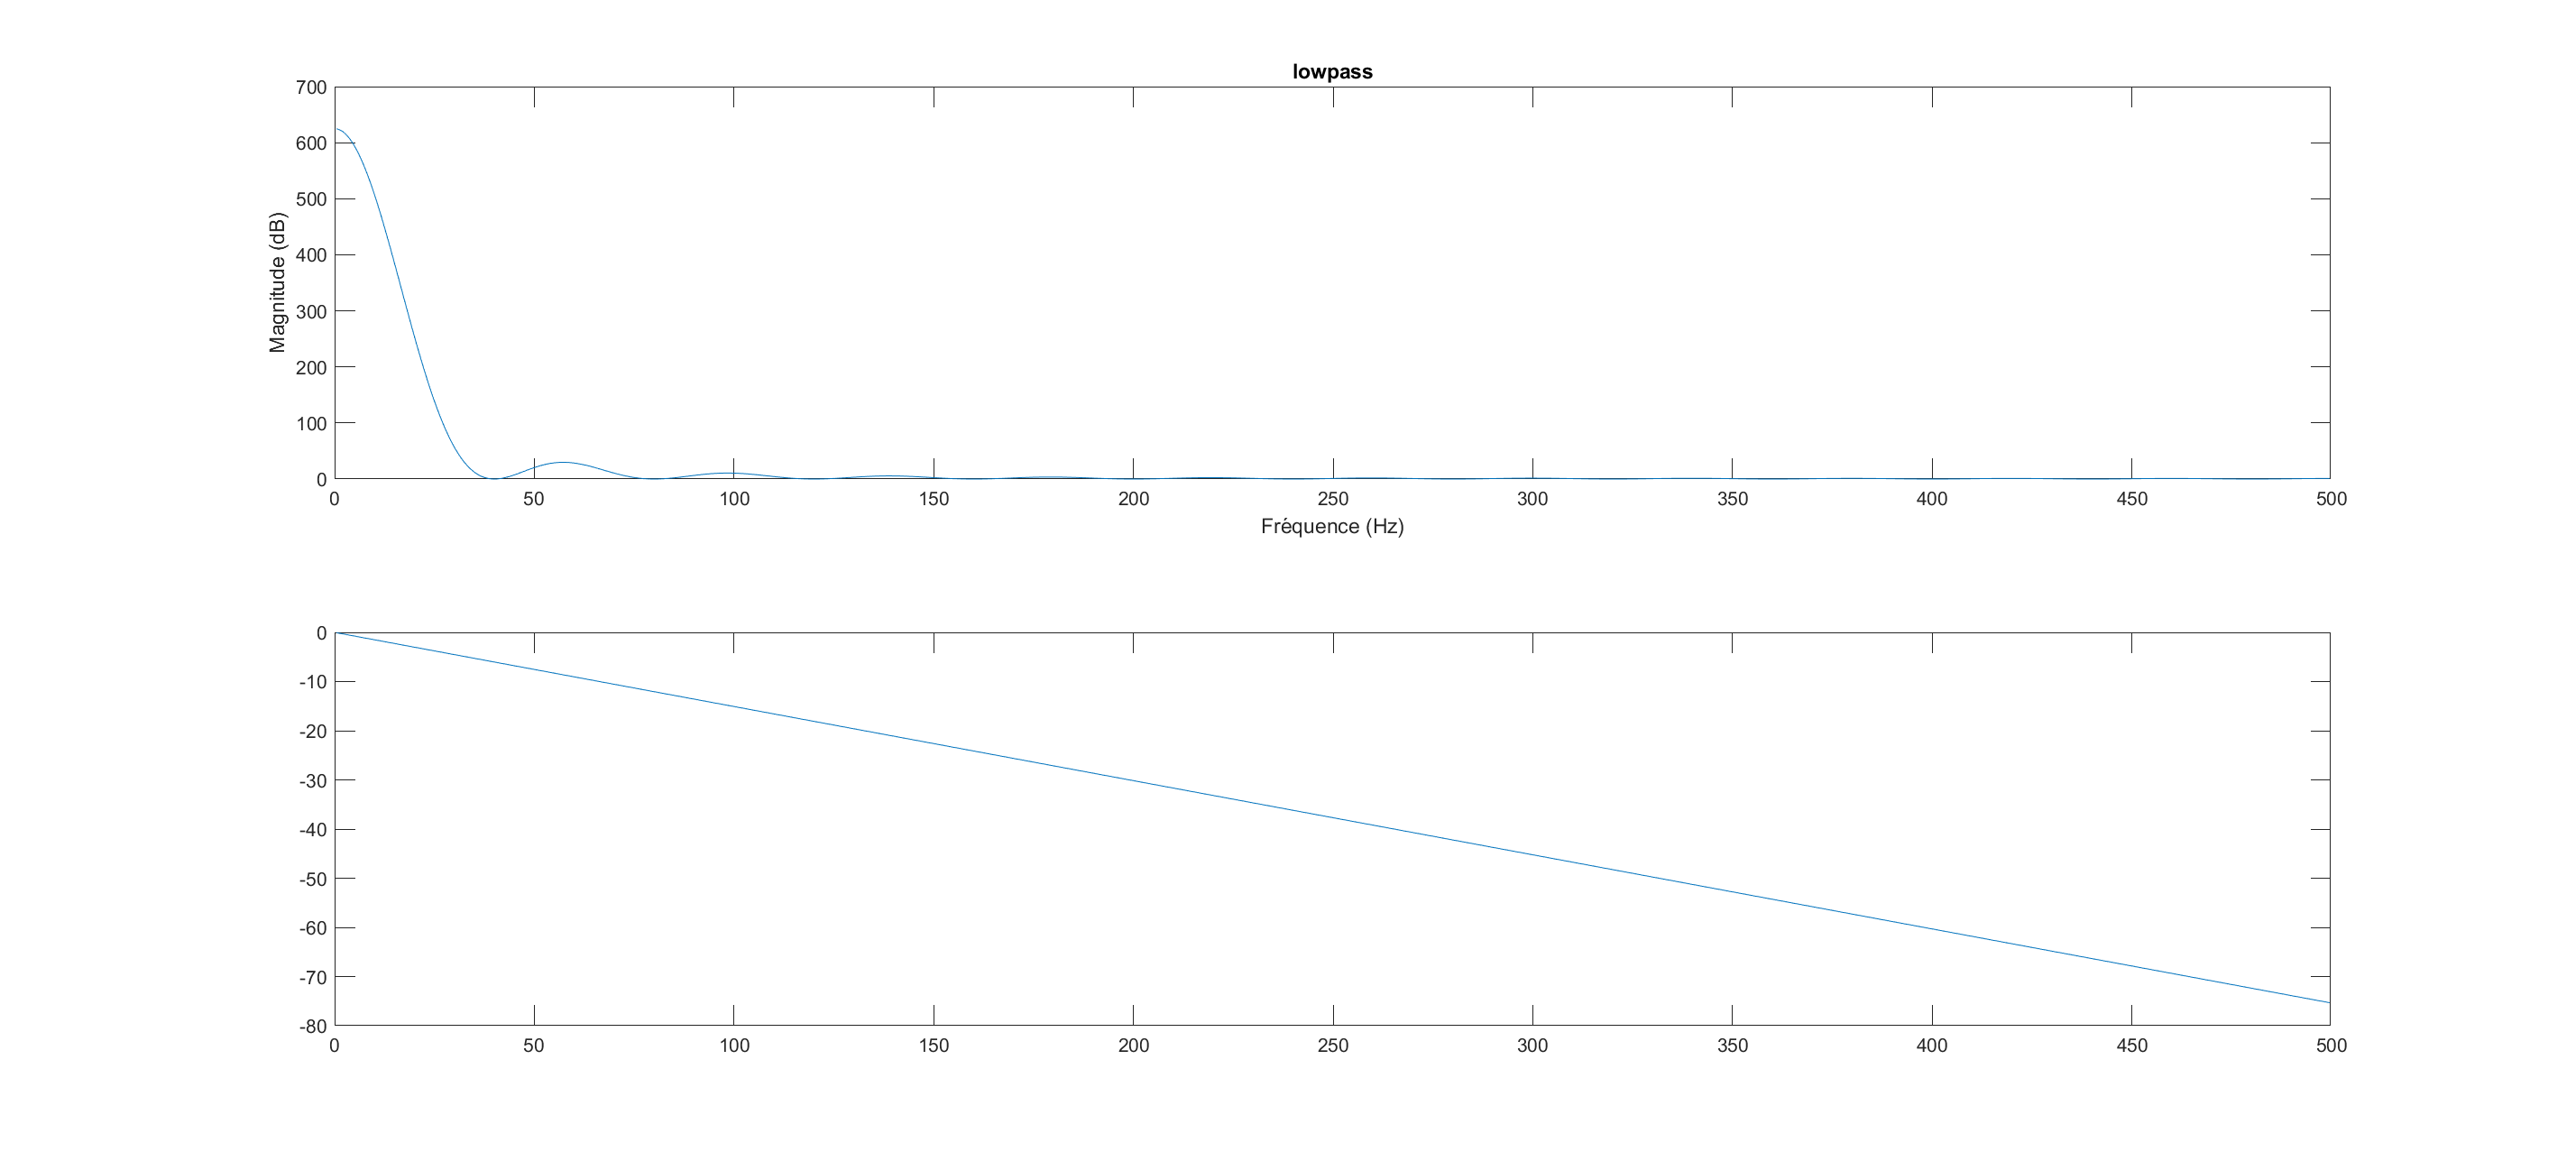
\includegraphics[width=.8\linewidth]{fig4}  
  \caption{passe-bas}
  \label{fig:sub-first}
\end{subfigure}
\begin{subfigure}{.5\textwidth}
  \centering
  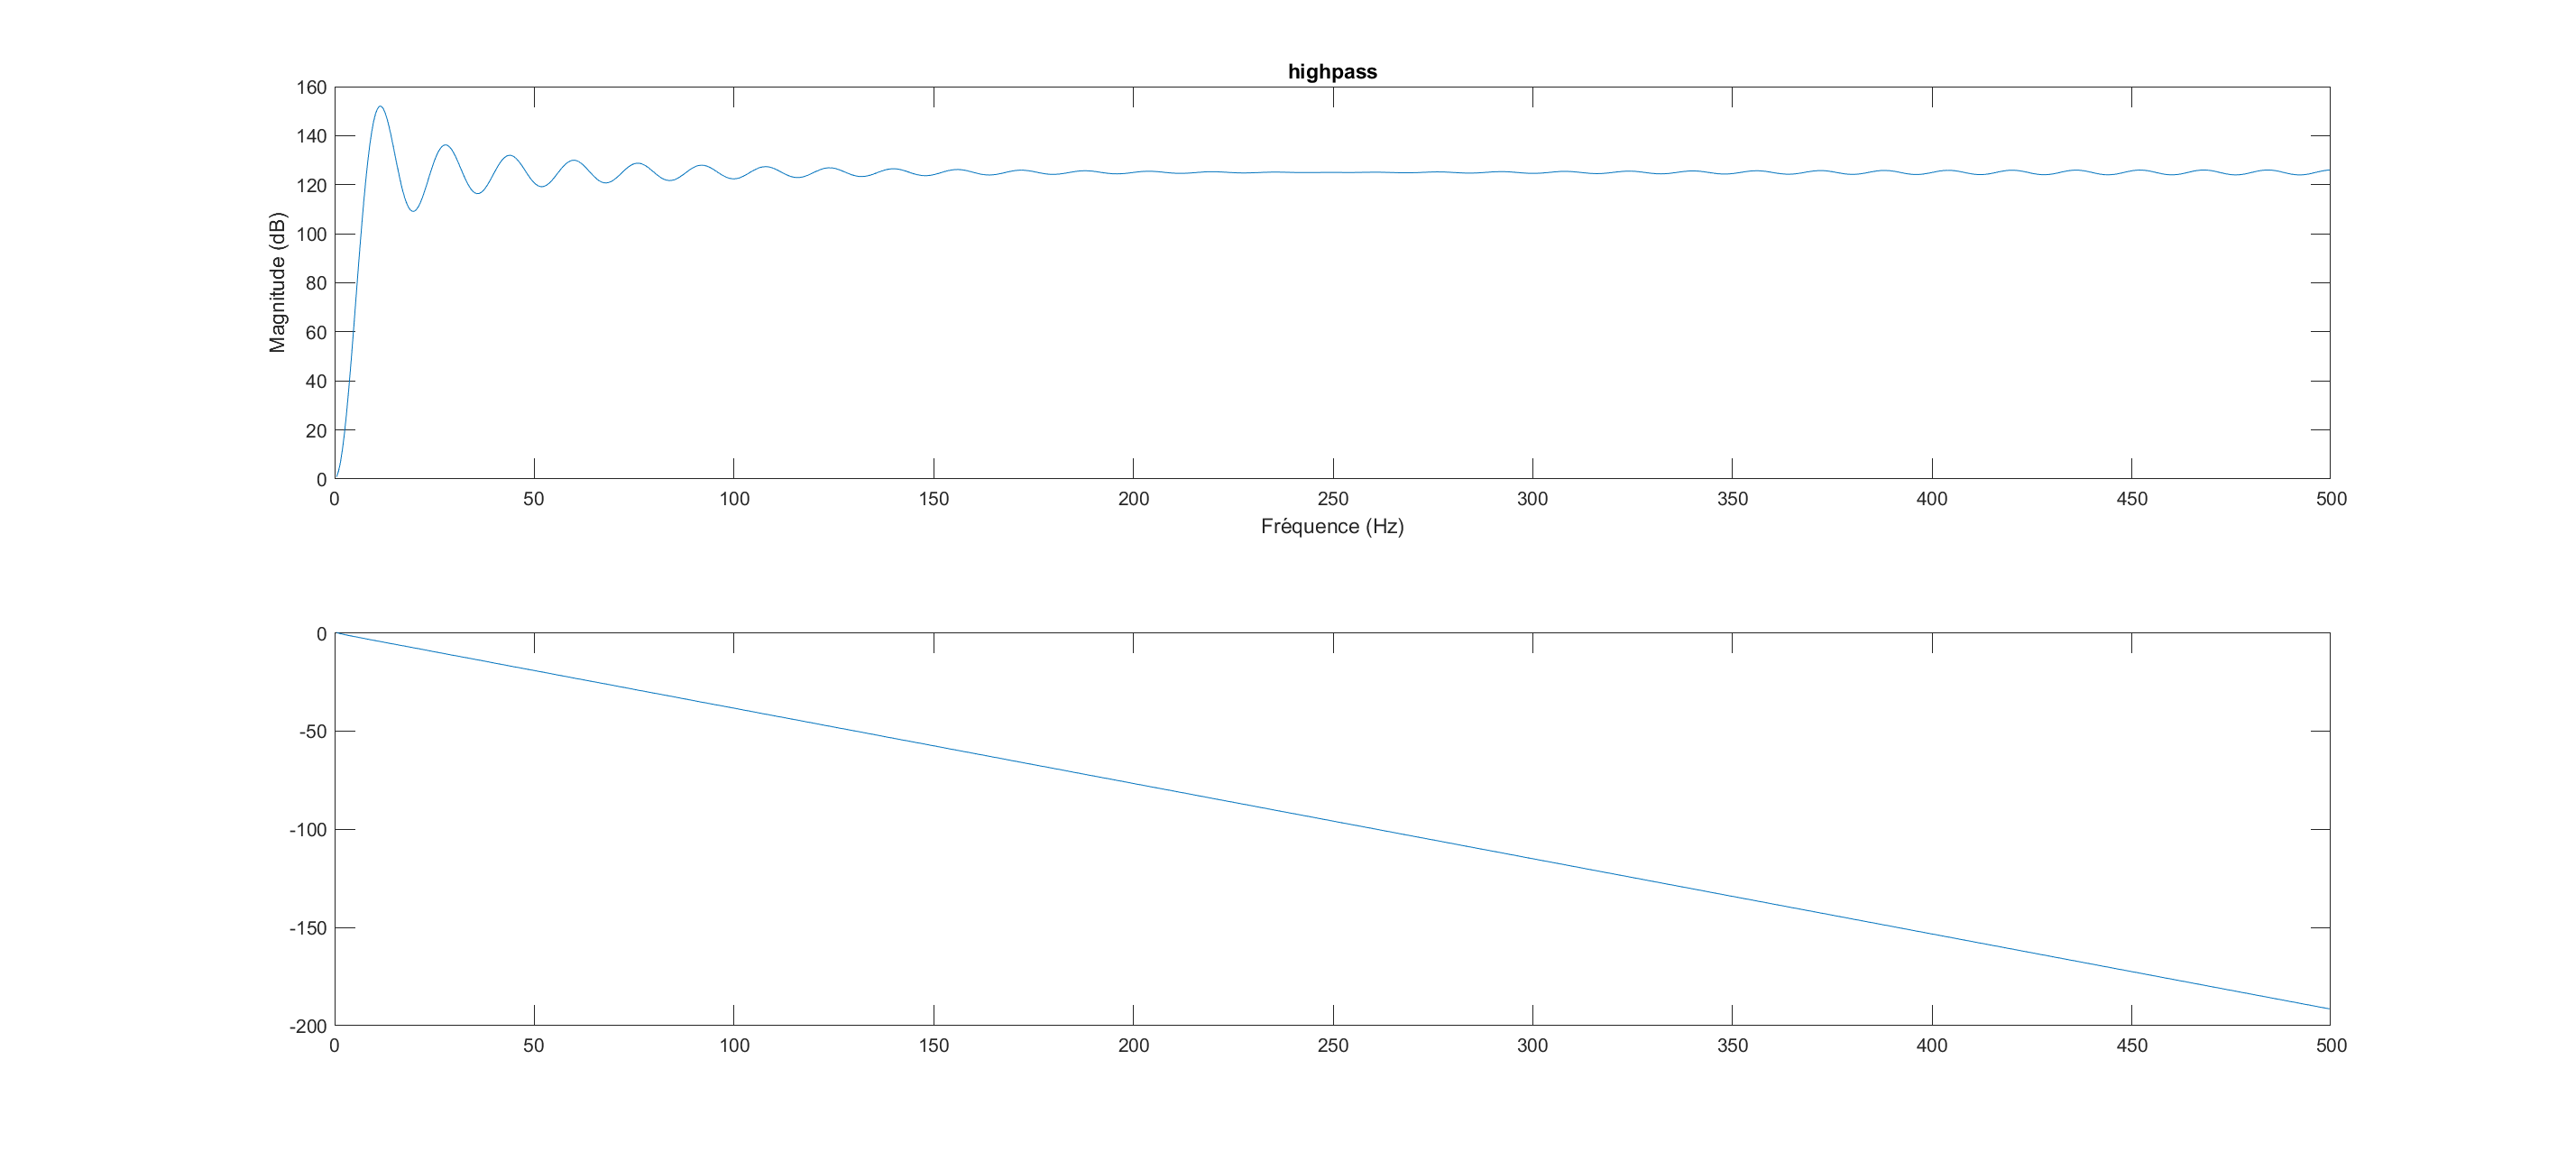
\includegraphics[width=.8\linewidth]{fig5}  
  \caption{passe-haut}
  \label{fig:sub-second}
\end{subfigure}

\newline

\begin{subfigure}{.5\textwidth}
  \centering
  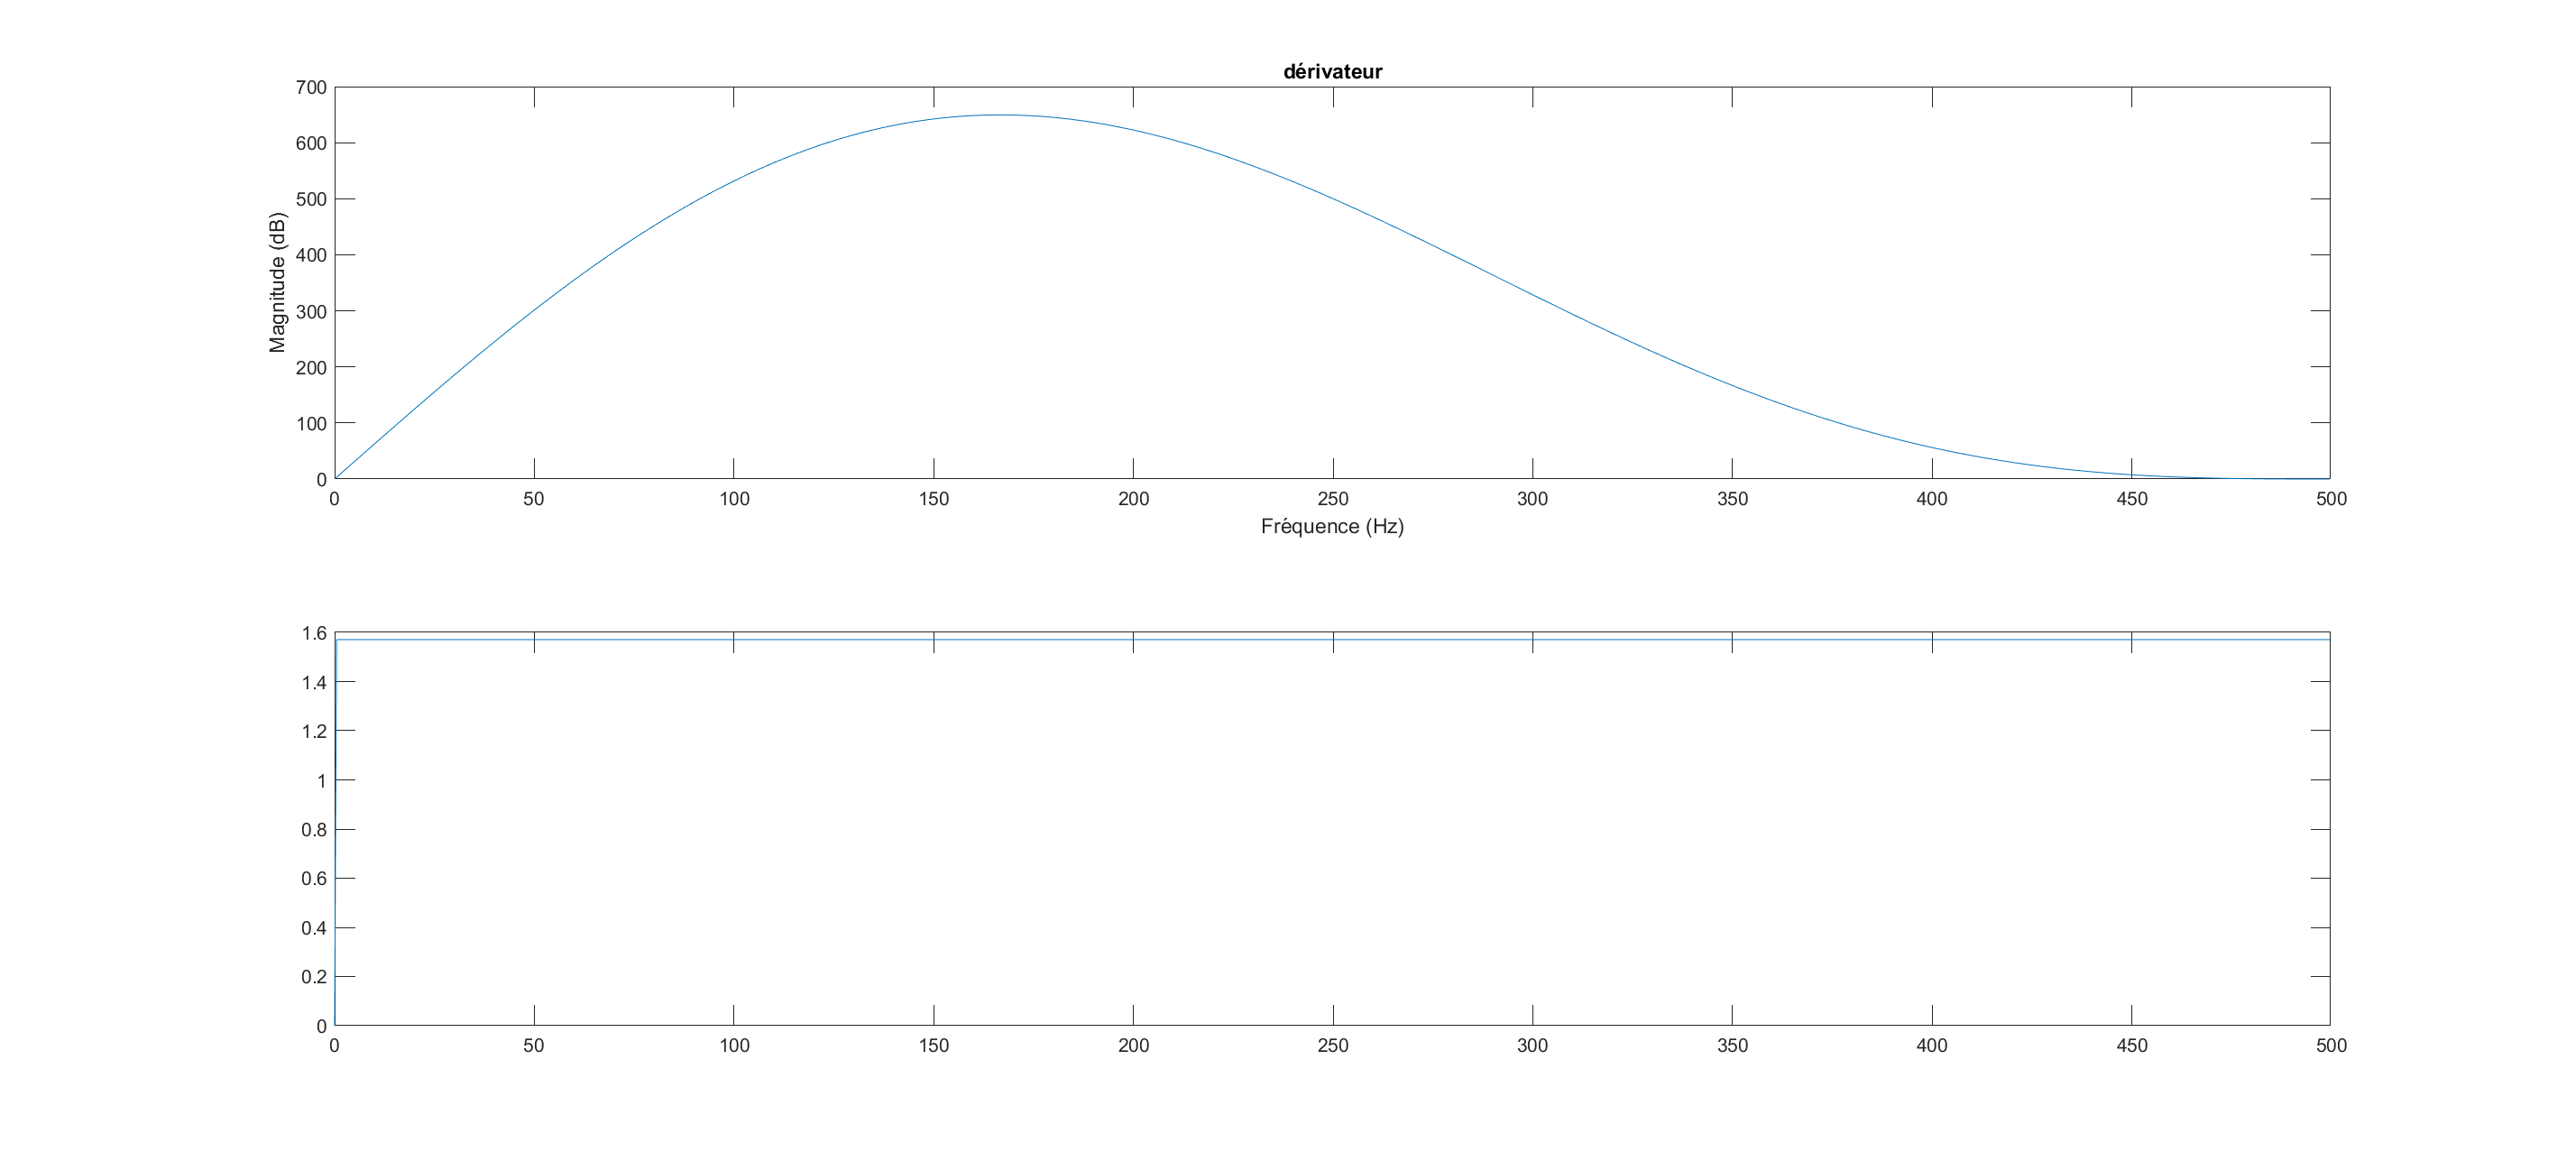
\includegraphics[width=.8\linewidth]{fig6}  
  \caption{MA}
  \label{fig:sub-third}
\end{subfigure}
\begin{subfigure}{.5\textwidth}
  \centering
  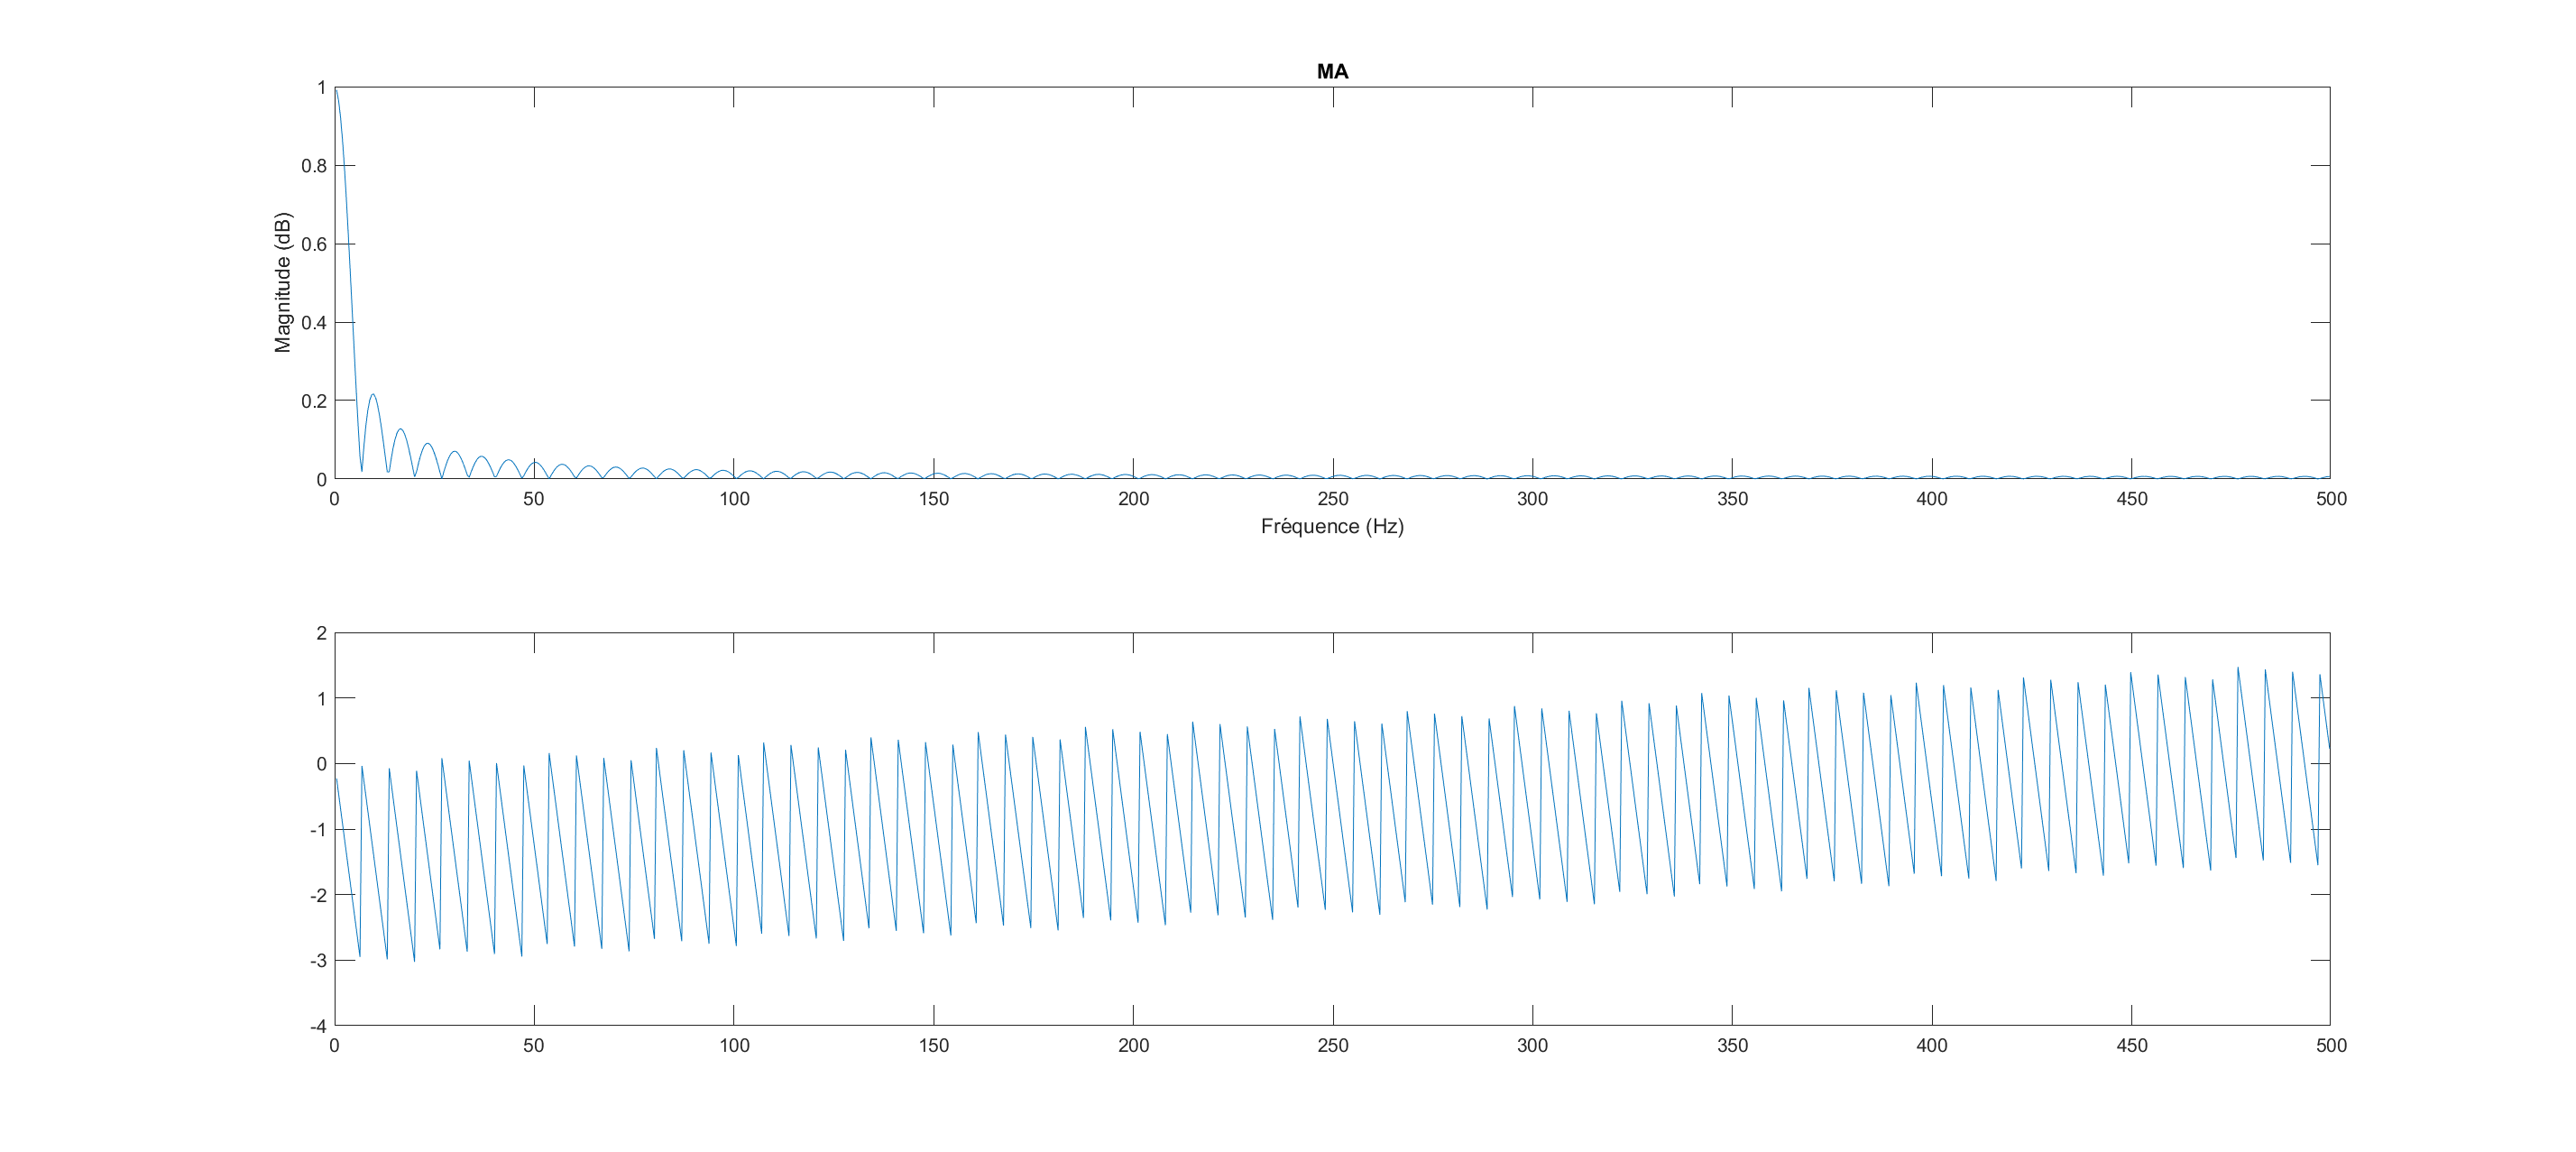
\includegraphics[width=.8\linewidth]{fig7}  
  \caption{Dérivateur}
  \label{fig:sub-fourth}
\end{subfigure}
\caption{Réponses fréquentielles}
\label{fig:fig}
\end{figure}

On observe alors que les tracés pour les différents filtres ont bien les allures attendues, 
avec les bonnes fréquences de coupure et une phase linéaire pour le passe-bas et le 
passe-haut.

Le terme $z^{-2}$ pour le filtre déviateur est nécessaire car il permet d'assurer la
causalité du filtre, ce qui assure que le système ne dépende pas du futur.

\subsubsection{Algorithm to detect R peaks}

Représentons les résultats obtenus par les algorithmes de détection de pics R :

\begin{figure}[H]
    \caption{Résultats des algorithmes}
    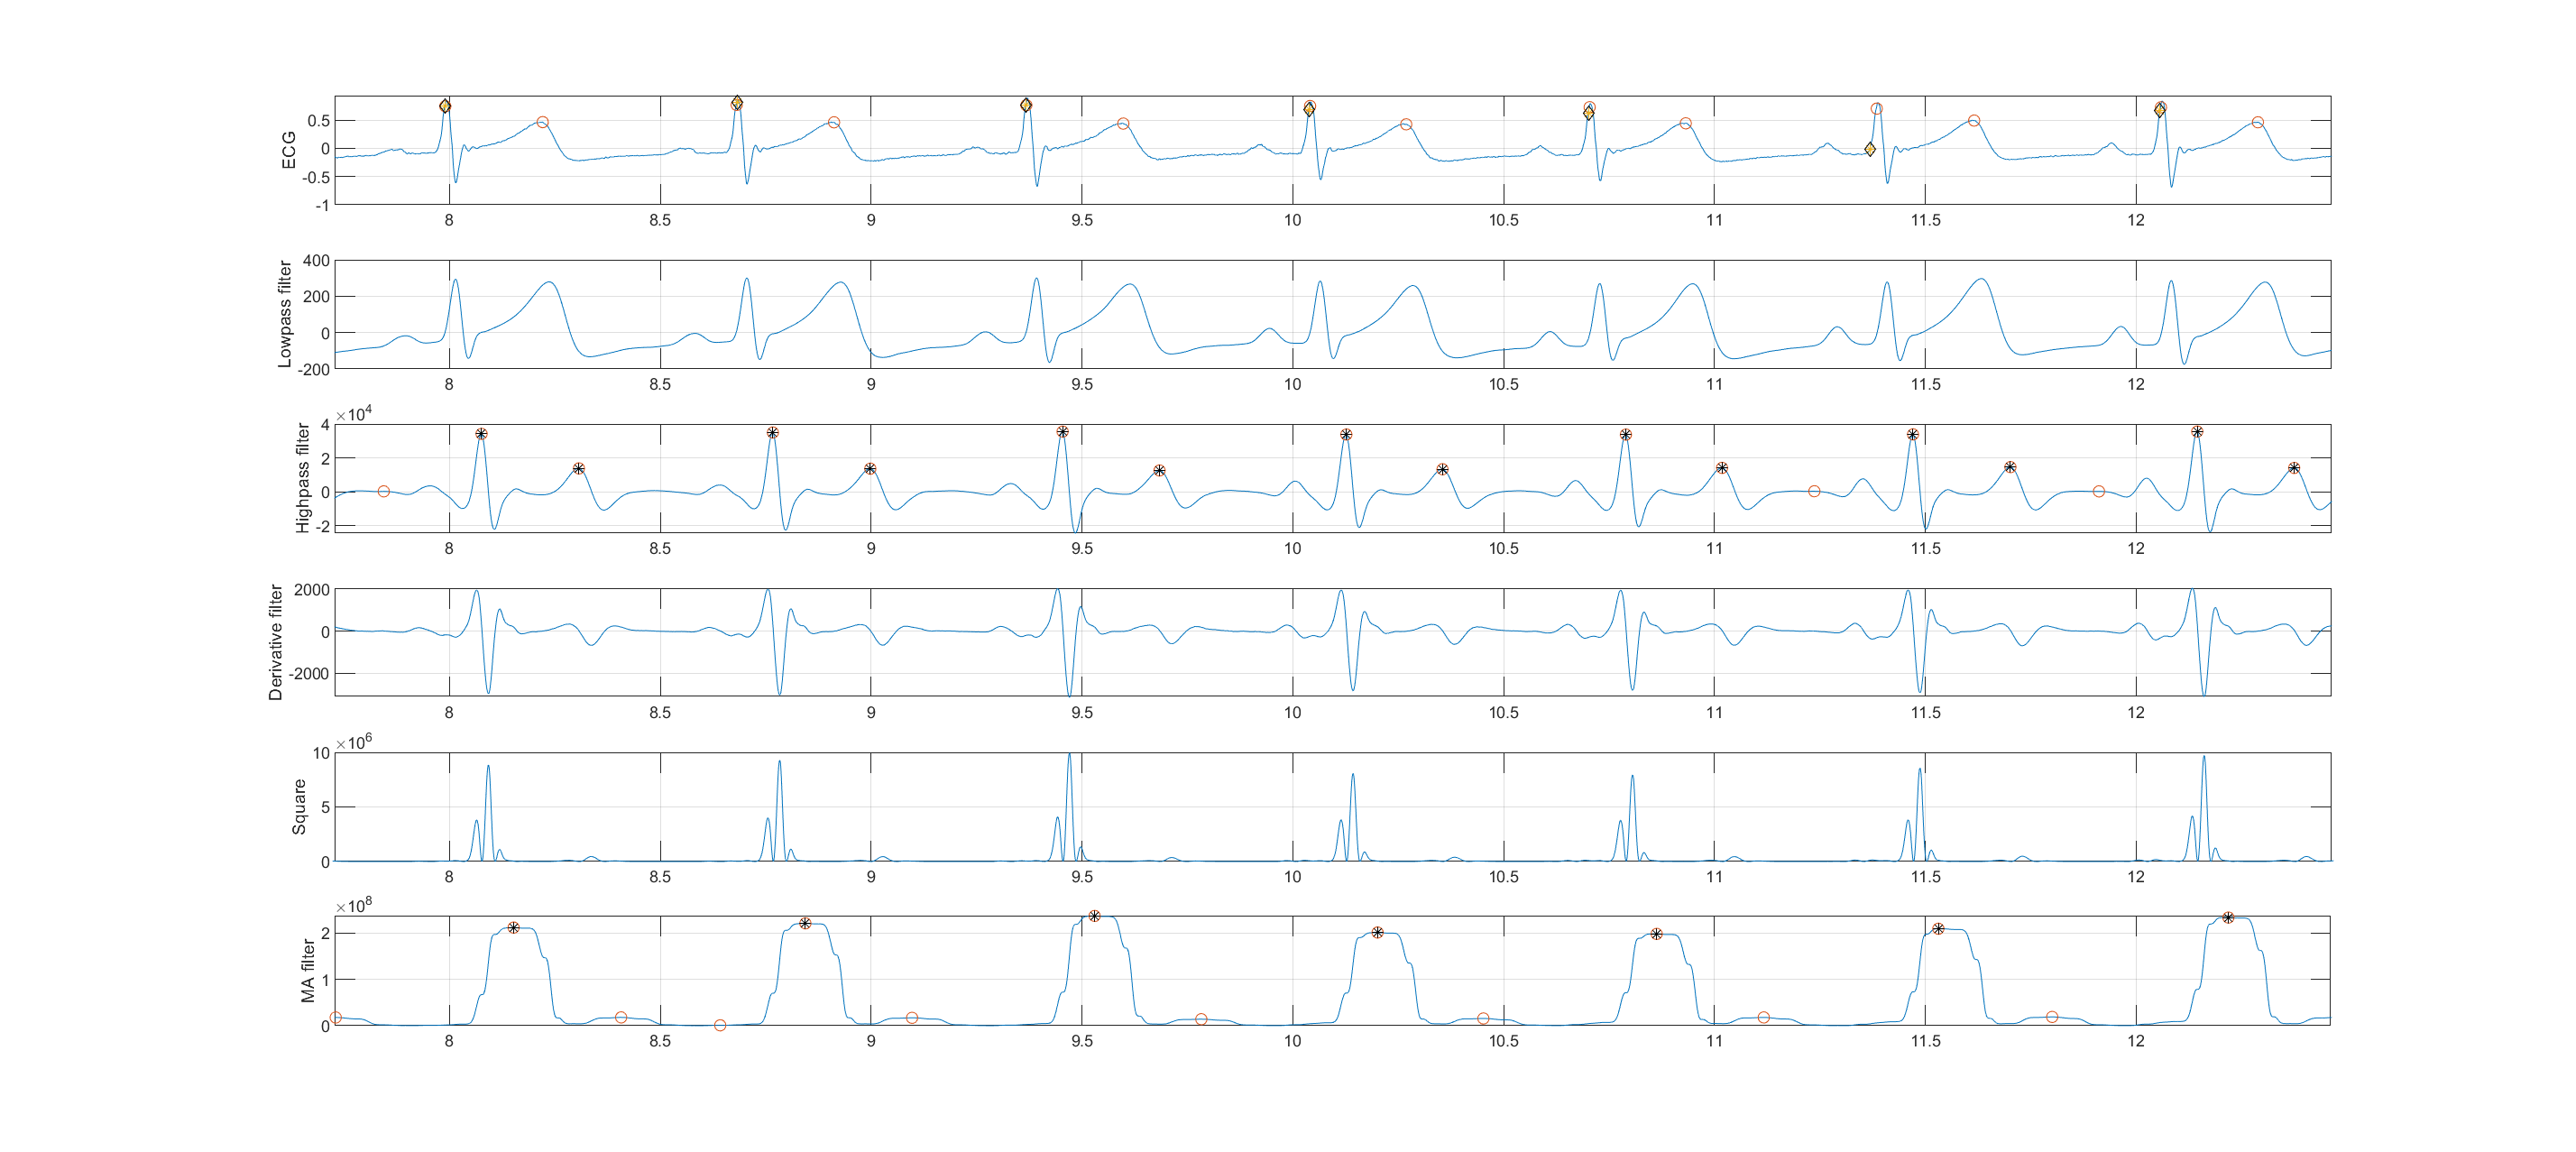
\includegraphics[width=\textwidth]{fig8}
    \centering
\end{figure}

On observe alors sur la figure ci-dessus que :

\begin{itemize}
    \item{Chacun des deux algorithmes pris séparément détecte les pics R mais aussi les
            pics T}
    \item{La prise en compte des deux algorithmes permet d'éliminer le détection des pics
            T}
    \item{La détection n'est quand même pas parfaite. On voit que les pics sont parfois
            détectés avec un léger décalage}
\end{itemize}

Ainsi, ces algorithmes simples à mettre en œuvre et peu couteux en calculs permettent 
d'obtenir des résultats satisfaisants sur un ECG sain.

\section{Fetal ECG extraction}

\subsection{Spatial filtering: $\pi$CA}

\subsection{ECG denoising by extended Kalman filtering}

\section*{Conclusion}

Ainsi,

\end{document}
